\chapter{7. Factory Pattern}
\section{Giới thiệu}
\subsection{Đặt vấn đề}
Vấn đề.
\begin{itemize}
    \item Làm thế nào một ứng dụng có thể độc lập với cách các đối tượng của nó được tạo ra?
    \item Làm thế nào một lớp có thể độc lập với cách các đối tượng mà nó yêu cầu được tạo ra?
    \item Làm thế nào có thể tạo mối quan hệ của các đối tượng liên quan hoặc phụ thuộc?
\end{itemize}
Việc tạo các đối tượng trực tiếp bên trong lớp yêu cầu các đối tượng là không linh hoạt vì nó gán lớp với các đối tượng cụ thể và khiến nó không thể thay đổi việc khởi tạo sau này một cách độc lập với (mà không cần phải thay đổi) lớp. Nó ngăn lớp không thể sử dụng lại nếu các đối tượng khác được yêu cầu và nó làm cho lớp khó kiểm tra vì không thể thay thế các đối tượng thực bằng các đối tượng giả.\\
Factory Pattern mô tả cách giải quyết các vấn đề như vậy.

\subsection{Mục đích sử dụng}
Mục đích sử dụng:
\begin{itemize}
    \item Giúp việc khởi tạo các đối tượng mà che giấu đi xử lí logic của việc khởi tạo đó. Người dùng không biết logic thực sự được khởi tạo bên dưới phương thức factory.
    \item Mẫu thiết kế này cho phép các lớp con chọn kiểu đối tượng cần tạo.
    \item Nó thúc đẩy sự liên kết lỏng lẻo bằng cách loại bỏ sự cần thiết phải ràng buộc các lớp cụ thể vào code. Nghĩa là code chỉ tương tác với interface hoặc lớp abstract, để nó sẽ làm việc với bất kỳ lớp nào implements interface đó hoặc extends lớp abstract.
    \item Factory Pattern giúp giảm sự phụ thuộc giữa các module: cung cấp 1 hướng tiếp cận với Interface thay vì các implement. Giúp chương trình độc lập với những lớp cụ thể mà chúng ta cần tạo 1 đối tượng, code ở phía client sẽ không bị ảnh hưởng khi thay đổi logic ở factory hay subclass.
    \item Việc kế thừa dễ dàng hơn: khi cần kế thừa, chỉ việc tạo ra những subclass và implement thêm vào factory method.
    \item Dễ dạng quản lý life cycle của các đối tượng được tạo bởi Factory Method Pattern.
    \item Thống nhất về mặt naming convention: giúp cho các developer có thể hiểu về cấu trúc source code.
\end{itemize}

\section{Định nghĩa và mô hình cấu trúc}
\subsection{Định nghĩa}
Mẫu thiết kế Factory Method xác định một giao diện để tạo một đối tượng, nhưng cho phép các lớp con
quyết định lớp sẽ khởi tạo. Factory Method cho phép một class trì hoãn việc khởi tạo thành các lớp subclass.
Mẫu thiết kế Abstract Factory cung cấp một giao diện để tạo các họ có liên quan hoặc các đối tượng phụ thuộc mà không chỉ định các lớp cụ thể của chúng
\subsection{Mô hình cấu trúc}
\begin{figure}[!htb]
    \centering
    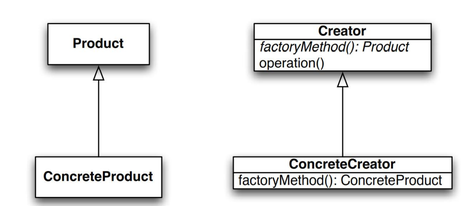
\includegraphics[width=\textwidth]{fig/Factory/structure_factory_method.png}
    \caption{Mô hình cấu trúc Factory Method}
    \label{fig:structure_factory_method}
\end{figure}
\begin{figure}[!htb]
    \centering
    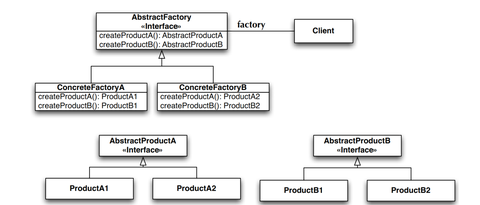
\includegraphics[width=\textwidth]{fig/Factory/structure_factory.png}
    \caption{Mô hình cấu trúc Factory Pattern}
    \label{fig:structure_factory}
\end{figure}
\begin{itemize}
    \item Super Class: môt super class trong Factory Pattern có thể là một interface, abstract class hay một class thông thường.
    \item Sub Classes: các sub class sẽ cài đặt các phương thức của super class theo nghiệp vụ riêng của nó.
    \item Factory Class: một class chịu tránh nhiệm khởi tạo các đối tượng sub class dựa theo tham số đầu vào. Lưu ý: lớp này là Singleton hoặc cung cấp một public static method cho việc truy xuất và khởi tạo đối tượng. Factory class sử dụng if-else hoặc switch-case để xác định class con đầu ra.
\end{itemize}
\section{Cách cài đặt}
Cài đặt Factory Pattern qua 1 bài toán thực tế theo sơ đồ dưới đây.

\begin{figure}[!htb]
    \centering
    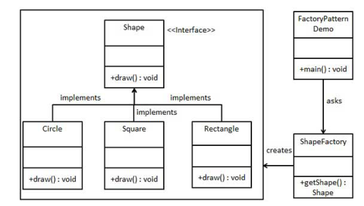
\includegraphics[width=\textwidth]{fig/Factory/example_structure_factory.png}
    \caption{Mô hình ví dụ}
    \label{fig:example_structure_factory}
\end{figure}
Cách cài đặt.
\\Link code cài đặt:
\url{https://github.com/nanhus/OOP-DesginPatten/tree/master/source/factory}\\

Bước 1: Tạo 1 giao diện.
\begin{figure}[!htb]
    \centering
    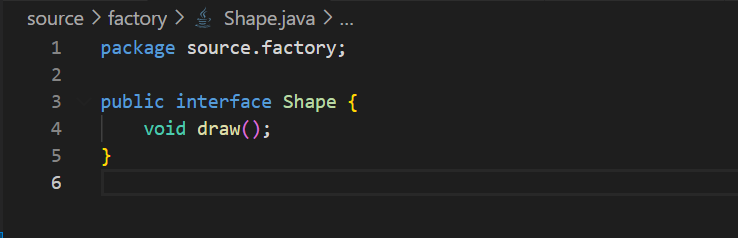
\includegraphics[width=\textwidth]{fig/Factory/shape_class.png}
    \caption{Shape interface}
    \label{fig:shape_class}
\end{figure}

\newpage
Bước 2: Tạo các đối tượng cụ thể cài đặt giao diện Shape.
\begin{figure}[!htb]
    \centering
    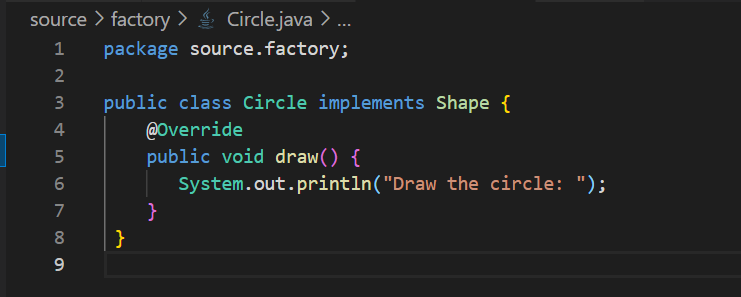
\includegraphics[width=\textwidth]{fig/Factory/circle_class.png}
    \caption{Circle Class}
    \label{fig:circle_class}
\end{figure}

\begin{figure}[!htb]
    \centering
    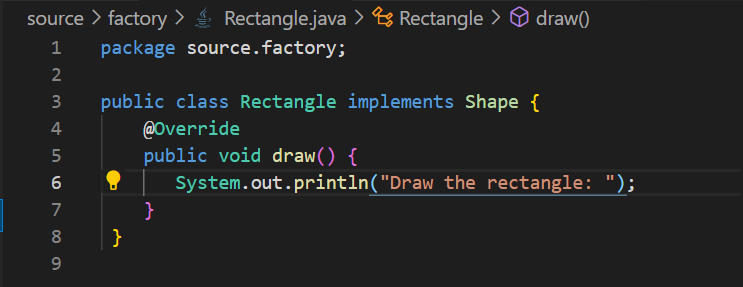
\includegraphics[width=\textwidth]{fig/Factory/rectangle_class.png}
    \caption{Rectangle Class}
    \label{fig:rectangle_class}
\end{figure}

\begin{figure}[!htb]
    \centering
    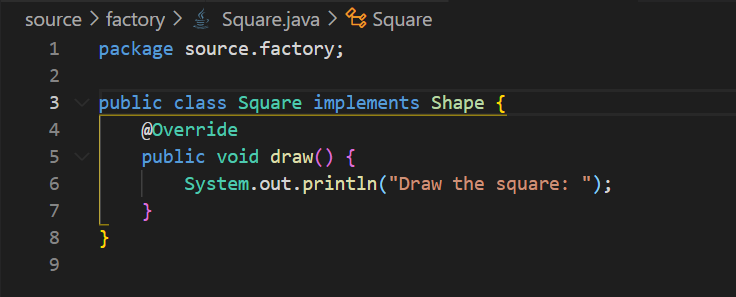
\includegraphics[width=\textwidth]{fig/Factory/square_class.png}
    \caption{Square Class}
    \label{fig:square_class}
\end{figure}

\newpage
Bước 3: Tạo một class ShapeFactory để tạo đối tượng của lớp cụ thể dựa trên thông tin đã cho.

\begin{figure}[!htb]
    \centering
    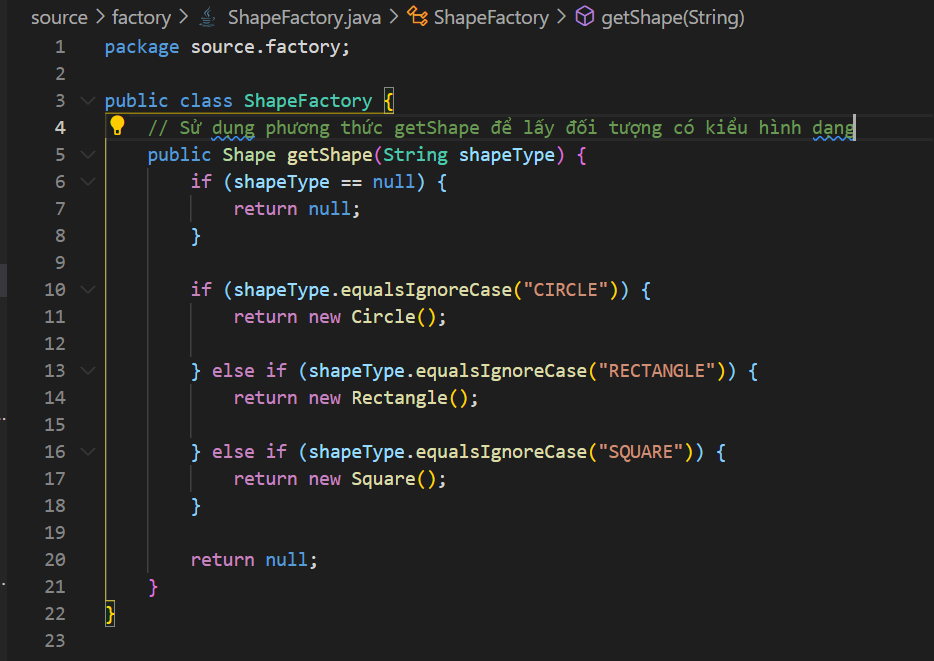
\includegraphics[width=\textwidth]{fig/Factory/shape_factory_class.png}
    \caption{Shape Factory Class}
    \label{fig:shape_factory_class}
\end{figure}

Bước 4: Sử dụng Factory để lấy đối tượng của lớp cụ thể bằng cách truyền một thông tin như kiểu.

\begin{figure}[!htb]
    \centering
    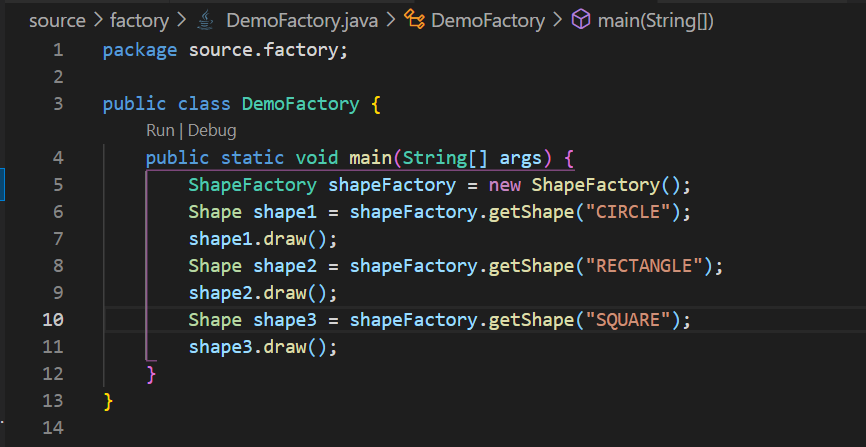
\includegraphics[width=\textwidth]{fig/Factory/demo_factory_class.png}
    \caption{Demo Factory class}
    \label{fig:demo_factory_class}
\end{figure}

\newpage
Output:
\begin{figure}[!htb]
    \centering
    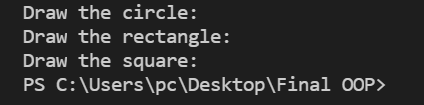
\includegraphics[width=\textwidth]{fig/Factory/factory_output.png}
    \caption{Output}
    \label{fig:factory_output}
\end{figure}

\section{Ví dụ thực tế}
\begin{itemize}
    \item Áp dụng quản lí các mặt hàng
    \item JDK: java.util.Calendar, ResourceBundle, NumberFormat, …
    \item BeanFactory trong Spring Framework.
    \item SessionFactory trong Hibernate Framework.
    \item Nó định nghĩa các Abstract Factory trong WidgetKit và DialogKit để tạo ra các đối tượng giao diện người dùng có giao diện cụ thể.
    \item Sử dụng mẫu Abstract Factory để đạt được tính di động trên các hệ thống khác nhau (ví dụ: X Windows và SunView). Lớp trừu tượng WindowSystem xác định giao diện để tạo đối tượng đại diện cho tài nguyên hệ thống cửa sổ (ví dụ: MakeWindow, MakeFont, MakeColor).
\end{itemize}

